\section{Neural Networks}
\label{sec:neural_network}

In this section a brief outline on the neural network architectures used in this work is given. It will be explained how the neural network works in general and how it is trained, but also some specific details about the architectures used in this work. 

\subsection{Neural Network Basics}

A neural network is a mathematical model that achieves statistical generalization drawing inspiration from the human brain. It is possible to define it as a function that maps an input to an output, given a set of parameters \( \bm{\theta} \). The function \( \hat{y} = f(\bm{x}; \bm{\theta}) \) is obtained by composing a series of functions \( f_i \) called layers, where each layer is defined as
\begin{equation}
    f_i = \sigma(W_i f_{i-1} + b_i)
\end{equation}
where \( W_i \) is the weight matrix, \( b_i \) is the bias vector and \( \sigma \) is the activation function. The activation function is a non-linear function that allows the network to learn complex patterns in the data. 

A neural network exists in function of a dataset \( \mathcal{D} = \{(\bm{x}_i, \bm{y}_i)\}_{i=1}^N \), where \( \bm{x}_i \) is the input and \( \bm{y}_i \) is the output. The final goal is to find the set of parameters \( \bm{\theta} \) that minimizes the loss function \( \mathcal{L} \), defined as some metric of the difference between the predicted output and the true output. The loss function:
\begin{equation}
    \mathcal{L} = \frac{1}{N} \sum_{i=1}^N L(f(\bm{x}_i; \bm{\theta}), \bm{y}_i)
\end{equation}
where \( L \) is the loss function, which can be the various metrics. The loss function is minimized using an optimization algorithm, so that the objective is to find
\begin{equation}
    \bm{\theta}^* = \argmin_{\bm{\theta}} \mathcal{L}
\end{equation}
which is the best set of parameters that minimizes the loss function.

The full algorithm is the following one:
\begin{algorithm} 
    \caption{Training of a neural network}
    \begin{algorithmic}
        \State Initialize the parameters \( \bm{\theta} \)
        \While{epoch < max\_epochs}
            \For{mini-batch in dataset}
                \State Perform forward pass computing \( f(\bm{x}; \bm{\theta}) \)
                \State Compute the loss function \( \mathcal{L}(f(\bm{x}; \bm{\theta}), \bm{y}) \)
                \State Perform backward pass computing the gradients of the loss function
                \State Update the parameters using the gradients
            \EndFor
        \EndWhile
    \end{algorithmic}
\end{algorithm}

\subsection{Neural Network Architectures}
Inside this work three different architectures were used: a simple fully connected neural network, a convolutional neural network and a graph neural network. Now a brief overview of the three architectures is presented, to better understand their inner mechanisms.

\subsubsection{Fully Connected Neural Network}
The simplest architecture is the fully connected neural network. It is composed of a series of layers, where each neuron is connected to all the neurons of the previous layer. 
\begin{figure}
    \centering
    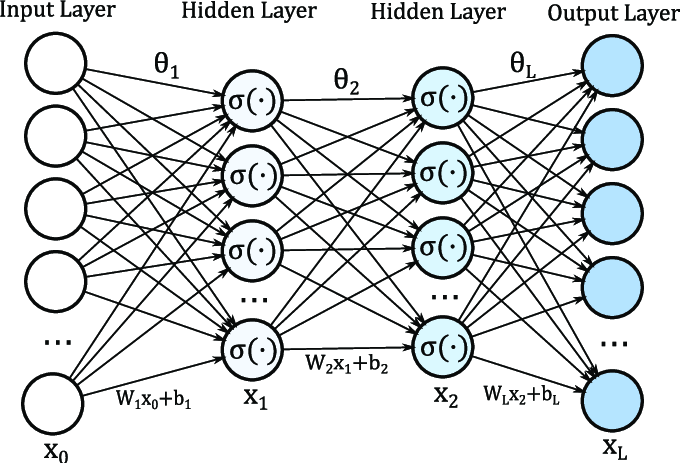
\includegraphics[width=0.5\textwidth]{fully_connected.png}
    \caption{Fully connected neural network from \cite{tonello2019machinelearningtipstricks}}
    \label{fig:fully_connected}
\end{figure}
The architecture is shown in \cref{fig:fully_connected}. The input is given by a vector \( \bm{x} \) and the output is given by a vector \( \bm{y} \). 
        